% Arara is a cross-platform automation tool to build pdf what follows are the build rules 
% arara: pdflatex: { synctex: on }
% arara: biber
% arara: makeglossaries
% arara: makeindex
% arara: pdflatex: { synctex: on }
% arara: pdflatex: { synctex: on }

\usepackage[utf8]{inputenc}     			% UTF8 encoding
\usepackage[margin=1in]{geometry}     		% margins 

\usepackage{hyperref} 						% href
\usepackage{graphicx}
\usepackage[font=small,labelfont=bf]{caption} % Required for specifying captions to tables and figures
\usepackage{verbatimbox}


\title{
	Mini Project 1 \\
	Machine learning, CS, MIU \thanks{Instructor: Anthony Sander}
}

\author{Baraa Mousa Noufal \and Ivan Krasowski Bissio}
\date{\today}

\begin{document}
\maketitle
\tableofcontents

\begin{abstract}
	\addcontentsline{toc}{section}{Abstract}

    Here goes the abstract

\end{abstract}

\section{About the Dataset}
Something about the dataset. What it is, where to find it (link), why we chose it...

\subsection{EDA: Exploratory Data Analysis}
Meaning of the data. Some visualization

\subsection{Data Preparation}
Feature selection (and why). How we encode categorical.

\subsection{Dataset Split}
How we split the dataset (train/test)

\section{Models}
% \subsection{Model 1: ...}
% \subsubsection{Presentation}
% \subsubsection{Training}
% \subsubsection{Validation}
% ... some more subsubsections
\subsubsection{Presentation}
KNearestNeighbors algorithm works by holding instances of training data and classifying by issuing a majority vote across "k" nearest neighbor of each point as to which class it belongs.

\subsubsection{Defining Parameters}
The data for training and validating is already defined by the Data Preparation step (80\% train, 20\% validation).\\
The representative parameter for KNN is \emph{n\_neighbors}: The number of neighboring instances taking part in the classification vote.\\

We trained the model on the default parameters (n\_neighbors=5) and achieved a 77\% accuracy on validation data.\\
We then attempted to tune the \emph{n\_neighbors} parameter using GridSearch across a range of values, it turned out the best value found by GridSearch for \emph{n\_neighbors} was 5 as well.\\
Next, we plotted the model score over a similar range, but scoring on the test dataset (rather than GridSearch).
\begin{center}
    \captionsetup{type=figure}
    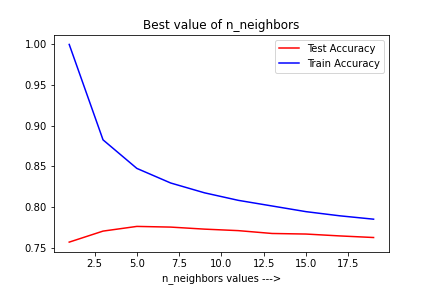
\includegraphics[width=250px]{knn_complexity.png}
    \captionof{figure}{Complexity Curve: \emph{n\_neighbors} value for KNN}
\end{center}
Observing the plot, it shows the same result as the validation accuracy starts to dip after \emph{n\_neighbors}=5.

\subsubsection{Model Evaluation}
Setting \emph{n\_neighbors}=5, we train another KNNClassifier and plot its learning curve as the data increases.
\begin{center}
    \captionsetup{type=figure}
    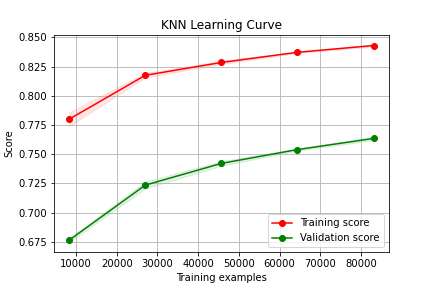
\includegraphics[width=250px]{learning_curve_knn.png}
    \captionof{figure}{Learning Curve for KNN}
\end{center}
Plot shows high variance but decreasing bias with more training data.

\subsection{Model 2: ...}
\subsubsection{Presentation}
\subsubsection{Training}
\subsubsection{Validation}
... some more subsubsections (like results)

... + other models (last model: Voting Classifier)

\section{AUCs}

\section{AutoML}
(+ new AUC, invluding AUC)


\section{Best model: model n}
Why the best
\subsection{PCA}
Does it improve?


% \subsection{Glossary}
% The \Gls{latex} typesetting markup language is specially suitable
% for documents that include \gls{maths}.\footnote{Don't forget to  run makeglossaries yourfile.tex}

% \subsubsection{Acronyms}
% Define in the glossary file as acronym and then use it as \gls{svm} or \gls{nn}.

% When we use the acronym again \gls{svm}. Notice the usage second time is converted to short form\footnote{check setacronymstyle setting}

\include{appendix.tex}
\end{document}
